\documentclass{article}
\usepackage{geometry}
\geometry{a4paper,scale=0.8}
\usepackage[utf8]{inputenc}
\usepackage{amssymb}
\usepackage{amsmath}
\usepackage[ruled,vlined]{algorithm2e}
\usepackage{float}
\usepackage{longtable,booktabs}
\usepackage{graphicx}
\usepackage{hyperref}
\usepackage{cite}
\usepackage{multicol}
\usepackage{authblk}
%\usepackage{algorithm} 
%\usepackage{algorithmic}
\usepackage{enumitem}
\usepackage[noend]{algpseudocode}
\newcommand\Algphase[1]{ \vspace*{-.7\baselineskip}\Statex\hspace*{\dimexpr-\algorithmicindent-2pt\relax}\rule{\textwidth}{0.4pt} \Statex\hspace*{-\algorithmicindent}\textbf{#1} \vspace*{-.7\baselineskip}\Statex\hspace*{\dimexpr-\algorithmicindent-2pt\relax}\rule{\textwidth}{0.4pt}}
\usepackage{adjustbox}
\usepackage{graphicx}
\usepackage[utf8]{inputenc}             
\usepackage[english]{babel}
\usepackage{tikz}
  \usetikzlibrary{shapes,arrows,fit,calc,positioning, decorations.pathreplacing}
  \tikzset{box/.style={draw, diamond, thick, text centered, minimum height=0.5cm, minimum width=1cm}}
  \tikzset{line/.style={draw, thick, -latex'}}
\usepackage{verbatim}
\usepackage{caption}
\setcounter{secnumdepth}{4}
\setcounter{tocdepth}{4}
\graphicspath{ {./figure/} }

\title{Analysis and classification of main risk factors causing stroke in Shanxi Province \footnote{Correspondence:  zhouxiaoshuang@sxmu.edu.cn, hhuang@uic.edu.cn} \footnote{J. Liu and Y. Sun contributed equally to this work.} }

\author[a]{Junjie Liu}
\author[b]{Yiyang Sun}
\author[c,e]{Jing Ma}
\author[a]{Jiachen Tu}
\author[a]{Yuhui Deng}
\author[a]{Ping He}
\author[d,a,e]{Huaxiong Huang} 
\author[f]{Xiaoshuang Zhou}
\author[c]{Shixin Xu}
\affil[a]{BNU-
HKBU United International College, Zhuhai, China}
\affil[b]{Duke Kunshan University, 8 Duke Ave, Kunshan, Jiangsu, China}
\affil[c]{Laboratory of Mathematics and Complex Systems (Ministry of Education), 
School of Mathematical Sciences, 
Beijing Normal University, Beijing 100875, China}
\affil[d]{Department of Mathematics and Statistics, York University, Toronto, Ontario, Canada}

\affil[e]{Research Center for Mathematics,
Beijing Normal University at Zhuhai, 519087, China}
\affil[e]{Department of Mathematics and Statistics, York University,
Toronto, Ontario, Canada} 
\affil[f]{Department of Nephrology, Shanxi Provincial People’s Hospital, Taiyuan, Shanxi, China;}
\date{}

\begin{document}

\maketitle

\textbf{Abstract}

\textbf{Background}: In China, stroke  is the first leading cause of death in recent years.  It  is a major cause of long-term physical and cognitive impairment, which bring great pressure on National Public Health System.  Evaluation of the risk of getting stroke is important for the prevention and treatment of stroke in China.

\textbf{Methods}: A data set with 2000 hospitalized stroke patients in 2018 and 27583 residents during the year 2017 to 2020 is analyzed in this study. Due to data incompleteness, inconsistency and non-structured formats, missing values in the raw data  are filled with -1 as an abnormal class. With the cleaned features, three models on risk levels of getting stroke are built by using machine learning methods. The importance of ``8+2'' factors from China National Stroke Prevention Project (CSPP) is evaluated via decision tree and random forest models. Except ``8+2'' factors the importance of features and SHAP\footnote{SHAP: SHapley Additive exPlanations} values for lifestyle information, demographic information and medical measurement are evaluated and ranked via random forest model. Furthermore, a logistic regression model is applied to evaluate the probability of getting stroke for different risk levels. 


\textbf{Results}: The risk of getting stroke for the 27583 residents is categorized and labeled with the CSPP's taxonomy: Low risk(11739 residents), Medium risk(7630 residents) and High risk(8214 residents). Among all ``8+2'' factors for the risk level of getting stroke, the decision tree model shows that top three features are  Hypertension (importance: $0.4995$), Physical Inactivity (importance: $0.08486$) and Diabetes Mellitus (importance: $0.07889$), and the random forest model shows that top three features are Hypertension (importance: $0.3966$), Hyperlipidemia (importance: $0.1229$) and Physical Inactivity (importance: $0.1146$). Except ``8+2'' factors the importance of features for lifestyle information, demographic information and medical measurement is evaluated via random forest model. It shows that top five features are Systolic blood pressure (importance: $0.3670$), Diastolic blood pressure (importance: $0.1541$), physical inactivity (importance: $0.0904$), Body Mass Index(BMI) (importance: $0.0721$) and Fasting Blood Glucose(FBG) (importance: $0.0531$). SHAP values show that Diastolic blood pressure, physical inactivity, Systolic blood pressure, BMI, smoking, FBG, and Triglyceride(TG) are positively correlated to the risk of getting stroke. High-density lipoprotein (HDL) is negatively correlated to the risk of getting stroke. Combining with the data of 2000 hospitalized stroke patients, the logistic regression model shows that the average probabilities of getting stroke are $7.20\%$ (with $95\%$ CI\footnote{CI: Confidence Interval}: $(6.65\%, 7.74\%)$) for the low-risk level patients,  $19.02\%$ (with $95\%$ CI: $(18.08\%, 19.96\%)$) for the medium-risk level patients and $83.89\%$ (with $95\%$ CI: $(82.93\%, 84.86\%)$) for the high-risk level patients.
\begin{comment}
\textbf{Conclusion}: Based on the census data in both communities and hospitals from Shanxi Province, in this paper, we investigate different stroke risk factors and their ranking. It shows that hypertension, physical inactivity (lack of sports), and overweight are ranked as the top three high stroke risk factors in Shanxi. The probability of getting a stroke is also estimated through our interpretable machine learning methods.
\end{comment}

\textbf{Conclusion}: Based on the census data in both communities and hospitals from Shanxi Province,   we investigate different risk factors of getting stroke and their ranking with interpretable machine learning models. The results show that Hypertension (Systolic blood pressure, Diastolic blood pressure), Physical Inactivity (Lack of sports), and Overweight (BMI) are ranked as the top three high risk factors of getting stroke in Shanxi province. The probability of getting stroke for a person can also be predicted via our machine learning model.


% \textbf{Clinical Perspective}\\
% \textbf{What is New?}

% The study quantifies the risk factors of stroke, and convert the scoring grades into probabilities, which make the prediction of stroke risk more intuitionistic. Besides, the logistic model is based on the current actual circumstance to predict the incidence promptly, which is more time-sensitive.\\
% \textbf{What are the Clinical Implications?}

% The evaluation methods we used confirm that hypertension, physical inactivity, and hyperlipidemia are the most important factors of causing the stroke. Diastolic blood pressure, systolic blood pressure, physical inactivity, BMI, smoking, FBG, TG, HDL, and family history of Stroke are the top ten factors when we only consider the lifestyle habits, demographic information, and medical measurement. 

\section{Introduction}\label{sec:Intro}
Stroke, an acute cerebrovascular disease, is caused by brain tissue damage due to abnormal blood supply to the brain with cerebrovascular blockage. It includes hemorrhagic stroke and ischemic stroke. According to the Global Burden of Disease, Injuries and Risk Factor Study and other researches \cite{liu2007stroke, roth2018global, zhou2019mortality}, stroke is the third leading cause of death in the world and the first in China. Recent studies from National Epidemiological Survey of Stroke in China(NESS-China) \cite{wang2017prevalence} show the prevalence of stroke in China during 2012-2013:

\begin{table}[H]
\small
\centering
\scalebox{0.7}{
\begin{tabular}{cccc}
\hline
\textbf{Region} & \textbf{Prevalence (Per 100000)} & \textbf{Incidence (per 100000)} & \textbf{Mortality (per 100000)} \\ \hline
Central China   & 1549.5                         & 326.1                                & 153.7                                \\
Northeast China & 1450.3                         & 365.2                                & 158.5                                \\
South China     & 624.5                          & 154.6                                & 65                                   \\ \hline
\end{tabular}}
\caption{Prevalence of Stroke in China}
\end{table}

Investigation into risk factors of getting stroke is essentially important for the prevention of stroke. Research shows that risk factors can be divided into two categories: reversible factors and irreversible factors.

Reversible factors mainly refer to unhealthy lifestyles such as smoking, excessive alcohol consumption and physical inactivity; while irreversible factors mainly refer to chronic diseases such as hypertension, diabetes, and hyperlipidemia. A number of researches on stroke risk analysis have been done for the European and American populations \cite{vartiainen2016predicting, lumley2002stroke}. However, they can not be directly applied to the Chinese population due to racial difference. 

In China, stroke-related research is mostly carried out on risk prediction models with pathogenic factors. The most widely used one is the 10-year risk prediction model using cardiovascular and cerebrovascular diseases to give probability of stroke and coronary heart disease incidence. The CHINA-PAR project (Prediction for ASCVD Risk in China) led by Gu Dongfeng's team \cite{yang2016predicting} proposed a revised model which considered not only the 10-year risk but also a lifetime-risk assessment.  By analyzing  data on the incidence of stroke in 32 of 34 provincial regions of China, Xu et al. \cite{xu2013there}  concluded that there is  a stroke belt in north and west China. 

%Xu et al. \cite{xu2013there} showed there is a stroke belt in china. It includes 9 provinces: Heilongjiang, Tibet, Jilin, Liaoning, Xinjiang, Hebei, Inner Mongolia, Bejing, and Ningxia.

In recent years, some machine learning methods have been applied to the stroke prediction. In 2010, a combination of Support Vector Machine and Cox Proportional Hazard Model was proposed  by Khosla et al.  \cite{khosla2010integrated}. Benjamin \cite{letham2015interpretable} implemented an interpretable method using Decision List with Bayesian Analysis to quantify the probability of stroke. Chi-Chun Lee's team \cite{hung2017comparing, hung2019development} compared multiple methods including Deep Neural Network in stroke prediction with Electronic Health Records (EHR). In their research, they focus on the patient's 3 year stroke rate and 8 year stroke rate. However, few of these studies modeled the early screening and prevention of stroke. 

 Evaluation of the risk of getting stroke is important for prevention and treatment of stroke in China. The China National Stroke Prevention Project (CSPP)\label{project:CSPP} proposed ``8 + 2" main risk factors in identifying Chinese residents' risk level of getting stroke \cite{yu2016csdc, li2019using,chao2021stroke}:

\begin{itemize}\label{factor:main-risk-factor}
    \setlength{\itemsep}{0pt}
    \setlength{\parsep}{0pt}
    \setlength{\parskip}{0pt}
    \item[1.] Hypertension
    \item[2.] Diabetes mellitus
    \item[3.] Heart disease(includes atrial fibrillation and valvular heart disease)
    \item[4.] Hyperlipidemia
    \item[5.] Family history of stroke
    \item[6.] Overweight
    \item[7.] Smoking
    \item[8.] Physical inactivity  
    \item[\textit{a.}] The history of stroke
    \item[\textit{b.}] The history of Transient Ischemic Attack (TIA)
\end{itemize}

With the above proposed ``8+2'' main risk factors, the risk level of getting stroke can be classified into:
\begin{itemize}
  \item[1.] \textbf{High risk:} having at least three factors from factor 1 to 8; or one of \textit{a} and \textit{b};
  \item[2.] \textbf{Medium risk:} having less than three risk factors from factor 1 to 8 with at least one being factor 1, 2 or 3; 
  \item[3.] \textbf{Low risk:} having less than three risk factors from factor 4 to 8.
\end{itemize}
 
 However, the ranking of the risk factors may present differently in different provinces. Based on the census data in both communities and hospitals from Shanxi Province, in this paper, we investigates different stroke risk factors and their ranking. It shows that hypertension, physical inactivity (lack of sports), and overweight are ranked as the top three high stroke risk factors in Shanxi. The probability of getting a stroke is also estimated through our interpretable machine learning methods. The study provides theoretical support for stroke prevention and control in Shanxi Province.
\begin{comment}
\subsection{Summary}
\begin{itemize}
    \setlength{\itemsep}{0pt}
    \setlength{\parsep}{0pt}
    \setlength{\parskip}{0pt}
    \item[1.] We rank the ``8+2" risk factors by using the Decision-Tree Model.
    \item[2.] The ranking of risk factors other than ``8+2" is given by using the Random-Forest Model.
    \item[3.] We quantify the probability of stroke incidence by using the logistic model. The features include lifestyle habits and the ``8+2" factors as these are easily accessible, and residents are able to use this model as a preliminary check by themselves. 
    \item[4.] In the discussion part, by comparing the 2016-data and 2017-2020 data, we propose a pipeline strategy in solving the data-imbalance problem.
    \item[5.] What's more, we investigate the influence of missing values with the permutation approach and using the average weight precision score and Recursive Feature Elimination(RFE) as the evaluation methods.
\end{itemize}

The Decision-Tree model shows that hypertension, physical inactivity, and hyperlipidemia are the top three factors in Shanxi province; The Random-Forest model shows that diastolic blood pressure, systolic blood pressure, physical inactivity, BMI, smoking, FBG, TG, HDL, and family history of Stroke are the top ten factors. The logistic model's result gives out the probability of stroke incidence: the average probability of stroke for the low-risk group is $0.1134$, the medium-risk group is $0.1935$, the high-risk group is $0.8528$, the stroke group is $0.9999$. 

Pipeline strategy has combined the One-vs.Rest and One-vs.One, which are two commonly used strategies in Multi-class classification. This strategy converts the multi-class classification into a step-by-step binary classification, and it is useful when the dataset is small and imbalanced. The results of the permutation approach and RFE show that diastolic blood pressure, physical inactivity, BMI, smoking, alcohol, HDL, and FBG are in order important factors when identifying the risk of stroke.
\end{comment}
\section{Materials and Methods}\label{sec:data-description}



\subsection{Dataset and Preprocessing}
 Our data is composed by two  survey datasets from 2017 to 2020:
%The datasets are composed by the Shanxi Provincial People's Hospital through a long period of survey and collection, which include:
\begin{itemize}[leftmargin=50pt]
    \setlength{\itemsep}{0pt}
    \setlength{\parsep}{0pt}
    \setlength{\parskip}{0pt}
    \item[Dataset 1:] Census in hospital: 2000 hospitalized stroke patients in 2018;
    \item[Dataset 2:] Census in community: 27583 residents during the year 2017 to 2020. This dataset is categorized and labeled with the CSPP's taxonomy: 
    \textit{Low risk (11739), Medium risk (7630) and High risk (8214).}
\end{itemize}


Each record in both datasets contains 177 features, not only providing information on the ``8+2" risk factors but also patients' other information:
\begin{table}[H]
\small
\centering
\begin{tabular}{ll}
\hline
\textbf{Feature   Name}      & \textbf{Example}                            \\ \hline
Demographic information      & Sex, Ethnicity, etc.                        \\
Lifestyle information        & Smoking, Alcohol consumption, etc.          \\
Medical measurement          & Blood pressure, fasting blood glucose, etc. \\
Surgery information          & history of surgery (PCI, CABG, CEA, CAS)    \\
Chronic diseases information & diagnosis times, what kinds of treatment    \\ \hline
\end{tabular}
\end{table}


 Data cleansing is a preparation process in data analysis by removing or correcting data that is corrupt or inaccurate.  The raw data in the above datasets needs to be cleaned due to data incompletion, inconsistence and non-structured formats which may lead to a failure of feature engineering. In this paper, missing values of a feature are filled with -1 as an abnormal class.  If there is over $60\%$ missing inside the column, we will delete it since the data from the column cannot provide much information.  Inconsistent values are found and corrected with prior medical knowledge. For instance, diastolic blood pressure should be lower than systolic blood pressure.  
 
 %Useful numerical values are extracted from non-structured format data. For instance, a float number 160 is extracted from ``160 cm'' in the feature ``Height''. 
 After the data cleansing, there are total 23289 records (low: 9718, mid: 6742, high: 5610) with 32 features in remains, shown in Table \ref{table:features}.  %The cleaned data will be used for our further study on features. 
\begin{table}[H]
\small
\centering
\begin{tabular}{lll}
\hline
\textbf{Class}                          & \textbf{Feature Name}    & \textbf{Data Type} \\ \hline
Lifestyle Information                   & Favor                    & Categorical        \\
Lifestyle Information                   & Alcohol                  & Categorical        \\
Lifestyle Information                   & Frequency of Vegetables  & Categorical       \\
Lifestyle Information                   & Frequency of Fruits      & Categorical       \\
Lifestyle Information                   & Meat and Vegetables      & Categorical       \\
Lifestyle Information                   & Medical Payment Method   & Categorical       \\
Demographic Information                 & Sex                      & Categorical        \\
Demographic Information                 & Age                      & Numerical          \\
Demographic Information                 & BMI                      & Numerical          \\
Demographic Information                 & Retire                   & Categorical        \\
Demographic Information                 & Height                   & Numerical          \\
Demographic Information                 & Weight                   & Numerical          \\
Demographic Information                 & Ethnicity                & Categorical        \\
Demographic Information                 & Occupation               & Categorical        \\
Demographic Information                 & Marital Status           & Categorical        \\
Demographic Information                 & Education Level          & Categorical        \\
Medical Measurement                     & TC                       & Numerical          \\
Medical Measurement                     & TG                       & Numerical          \\
Medical Measurement                     & HDL                      & Numerical          \\
Medical Measurement                     & LDL                      & Numerical          \\
Medical Measurement                     & HCY                      & Numerical          \\
Medical Measurement                     & FBG                      & Numerical          \\
Medical Measurement                     & Pulse                    & Numerical          \\
Medical Measurement                     & Systolic blood pressure  & Numerical          \\
Medical Measurement                     & Diastolic blood pressure & Numerical          \\
``8+2" Factor and Lifestyle Information  & Smoking                  & Categorical        \\
``8+2" Factor and Lifestyle Information  & Physical Inactivity      & Categorical        \\
``8+2" Factor and Medical Information    & Heart Disease            & Categorical        \\
``8+2" Factor and Medical Information    & Hypertension             & Categorical        \\
``8+2" Factor and Medical Information    & Hyperlipidemia           & Categorical        \\
``8+2" Factor and Medical Information    & History of Stroke        & Categorical        \\ 
``8+2" Factor and Medical Information    & Diabetes Melltius        & Categorical        \\
``8+2" Factor and Medical Information    & Family history of Stroke & Categorical        \\
``8+2" Factor and Medical Information    & History of Transient Ischemic Attack        & Categorical \\ \hline
\end{tabular}
\caption{Remaining features after Data Cleansing}
\label{table:features}
\end{table}

%\subsection{ Diagnosis   Criteria }

% The China National Stroke Prevention Project (CSPP)\label{project:CSPP} proposed ``8 + 2" main risk factors in identifying Chinese residents' risk level of getting stroke:

% \begin{itemize}\label{factor:main-risk-factor}
%     \setlength{\itemsep}{0pt}
%     \setlength{\parsep}{0pt}
%     \setlength{\parskip}{0pt}
%     \item[1.] Hypertension
%     \item[2.] Diabetes mellitus
%     \item[3.] Heart disease(includes atrial fibrillation and valvular heart disease)
%     \item[4.] Hyperlipidemia
%     \item[5.] Family history of stroke
%     \item[6.] Overweight
%     \item[7.] Smoking
%     \item[8.] Physical inactivity  
%     \item[\textit{a.}] The history of stroke
%     \item[\textit{b.}] The history of Transient Ischemic Attack (TIA)
% \end{itemize}

% With the above proposed ``8+2'' main risk factors, the risk level of getting stroke can be classified into:
% \begin{itemize}
%   \item[1.] \textbf{High risk:} having at least three factors from factor 1 to 8; or one of \textit{a} and \textit{b};
%   \item[2.] \textbf{Medium risk:} having less than three risk factors from factor 1 to 8 with at least one being factor 1, 2 or 3; 
%   \item[3.] \textbf{Low risk:} having less than three risk factors from factor 4 to 8.
% \end{itemize}


\begin{comment}
\subsection{Data Cleansing}
Data cleansing is a preparation process in data analysis by removing or correcting data that is corrupt or inaccurate. As the initial dataset we used contains, for example, incomplete data, error data, and unstructured data, which may lead to the problem of feature inaccuracy to data with defective features and incorrect data in the dataset. Hence, The data preprocessing procedure cannot be omitted.
\begin{itemize}[leftmargin=84pt]
    \setlength{\itemsep}{0pt}
    \setlength{\parsep}{0pt}
    \setlength{\parskip}{0pt}
    \item[Missing Values:] There are two common methods in solving the problem of missing values. The first one is to do the imputation with some certain statistic value such as the mean value and the median. The second one is using some statistical method, like regression, to generate the imputation values based on the other datapoints. What's more, if there are over $60\%$ missing inside a single feature, we would just delete the feature. In our case, it is difficult to get a predicted value for imputation. Hence, we choose the first method and do the imputation with mean value.
    \item[Error Data:] Error data is defined as the data violates common sense. Here is an example,  for a person, diastolic blood pressure should be lower than systolic blood pressure. However, inside the dataset, some respondent's diastolic blood pressure (140 mmHg) is larger than systolic blood pressure (87 mmHg). Based on the prior medical knowledge, the invalid data has been corrected: continued with the above example, we correct the data by  exchanging the two values: diastolic blood pressure equals 87 mmHg and the systolic blood pressure is 140 mmHg.
    \item[Unstructured data:] There are cases in our dataset where one data point contains either characters, integers and floating point numbers; we refer to this type of data as the unstructured data. For instance, ``160.0 cm" refers to the height of respondent, however, it contains both characters and floating number. Regular expressions are patterns used to match and extract some specific character combination from certain strings. We can extract the data we need from these non-structured data with the proper regular expression. 
\end{itemize}
\end{comment}

\begin{comment}
\subsection{Features Clustering}
%\textbf{Principal Component Analysis(PCA)} \cite{wold1987principal} is a mathematical transformation method that converts a given set of variables into a set of uncorrelated variables through linear transformation (the pairwise correlation coefficient is 0, or random variables whose sample vectors are perpendicular to each other).

%\textbf{Factor Analysis(FA)} \cite{rummel1988applied, mair2018factor} is a method of grouping variables according to their correlation magnitude so that variables within the same group are more correlated with each other, but variables in different groups are less correlated. For each group, it represents a basic structure, called common factor. It can be used to describe each component of the original observation in terms of the sum of a linear function of a minimum number of unmeasured so-called common factors.

Since the dataset involves numerous variables, it is difficult for us to discover the relationship between the different variables. In order to identify their inner connection and give us a full understanding of the feature, a feature clustering method is performed. VARCLUS, or PROC VARCLUS\cite{sanche2006variable,sarle1990varclus}, is a typical variable clustering algorithm proposed by SAS. This method draws on certain ideas from factor analysis and the hierarchical clustering method, which produces distinct clusters and these clusters can help to identify and discover the common factors. The process of VARCLUS can be illustrated as follow:

\par
\begin{multicols}{2}
\begin{figure}[H]
    \centering 
    \includegraphics[width=4.5cm]{figure/VARCLUS}
    \caption{VARCLUS Algorithm}
    \label{fig:VARCLUS}
\end{figure}

\par\noindent Table \ref{table:VARCLUS} below shows the result of variable clustering:
\begin{table}[H]
\small
\centering
\scalebox{0.55}{
\begin{tabular}{|c|c|c|c|c|}
\hline
\textbf{Cluster} & \textbf{Variable}          & \textbf{RS\_Own} & \textbf{RS\_NC} & \textbf{RS\_Ratio} \\ \hline
\multicolumn{5}{|c|}{\textbf{Others}}                                                                                      \\ \hline
0                & liver cirrhosis           & 0.5883                       & 0.00238     & 0.4127        \\ \hline
0                & renal nsufficiency       & 0.7121                      & 0.01052     & 0.2909        \\ \hline
0                & chronic headache          & 0.8361                      & 0.007616     & 0.1651        \\ \hline
\multicolumn{5}{|c|}{\textbf{Diabetes Mellitus \& Hyperlipidemia related}}                                                 \\ \hline
1                & frequency of blood glucose test       & 0.08715                      & 0.00223    & 0.91489        \\ \hline
1                &  do you know glucose tolerance test   & 0.005020                      & 0.00164   & 0.9966        \\ \hline
1                & FBG                        & 0.1420                      & 0.006782     & 0.8639         \\ \hline
1                & glycosylated hemoglobin   & 0.07881                      & 9.11E-05        & 0.9213         \\ \hline
1                & TG                         & 0.1237                      & 0.0024645     & 0.87847        \\ \hline
1                & TC                         & 0.7684                      & 0.0007821     & 0.2317        \\ \hline
1                & LDL                        & 0.7368                      & 0.002867     & 0.2640        \\ \hline
1                & HDL                        & 0.005240                    & 0.0005445     & 0.9953        \\ \hline
1                & CABG                       & 0.0009379                   & 0.0004786     & 0.9995        \\ \hline
1                & frequency of testing blood fat           & 0.03420                      & 0.003606     & 0.9693        \\ \hline
1                & pulse                      & 0.04749                      & 0.04751     & 1.000        \\ \hline
\multicolumn{5}{|c|}{\textbf{Heart Disease related}}                                                                       \\ \hline
2                & cardiac murmur            & 0.1623                      & 0.0044     & 0.8414         \\ \hline
2                & heart rate                & 0.3930                      & 0.05887     & 0.6450        \\ \hline
2                & CAS                        & 0.7747                      & 0.008916     & 0.2273        \\ \hline
2                & PCI                        & 0.5653                      & 0.003957     & 0.4364        \\ \hline
\multicolumn{5}{|c|}{\textbf{Hypertension \& Coronary Heart Disease related}}                                              \\ \hline
3                & coronary heart disease   & 0.01455                      & 0.0008248     & 0.9863        \\ \hline
3                & homocysteine               & 0.1754                      & 0.01165     & 0.8343        \\ \hline
3                & diastolic blood pressure & 0.6839                      & 0.006407     & 0.3182        \\ \hline
3                & systolic blood pressure  & 0.7594                      & 0.01004     & 0.2431        \\ \hline
\end{tabular}}
\caption{Variable Clustering Result}\label{table:VARCLUS}
\end{table}
\end{multicols}
The VARCLUS algorithm is often used in dimensional reduction, however, in our case, we see the result of clustering as a exploratory data analysis: by clustering the features in our dataset\footnote{by using a python package: \href{https://github.com/jingtt/varclushi}{varclushi}}, we can see that many of the medical measurement features are correlated and based on the medical knowledge, these clusters are related to different chronic diseases.

\section{Models}
Machine learning 
\end{comment}

%\section{\textcolor{blue}{Methods for Prediction and Interpretation}}\label{section:models}
%\section{Models and Model Interpretation}

%With the cleaned features, models on risk of getting stroke will be built through machine learning methods. In this paper, classification models such as decision tree and random forest are built to evaluate stroke risk levels, and regression models such as logistic regression are built to predict the probability of getting stroke. 

%The Predictive modelling is a process of training a mapping function $f(\cdot)$ from the input to the output, using the mapping function to predict the outcomes with the new input. The discovery of the input-output map is called function approximation. If the approximation is mapping the input to a discrete space, it is called classification; if the approximation is mapping the input to a continuous space, it is called regression. In this section, we start with some classification and regression methods which are used in our modelling part. \begin{comment}
%What's more, as our data contains multiple categories, some widely used classification strategies are used. \end{comment}In addition, we would introduce the model interpretation methods which are used in our model evaluation.

\subsection{Models}
\par\noindent\textbf{Decision-Tree} is a classic non-parametric machine learning algorithm. A tree is created through learning decision rules inferred from data features. Starting from the top root node, data are split into different internal nodes according to certain cutoff values in features, and then finally arrive the terminal leaf nodes which give the final classification result. ID3 \cite{quinlan1986induction} and CART \cite{breiman1984classification} are classic Decision-Tree algorithms which employ Information Gain and Gini Impurity from Entropy Theory \cite{pal1991entropy} as measurements in making best splitting rules.


\begin{comment}
It contains three elements: a root node, internal nodes, and leaf nodes. Starting from the root node at the top, data are split into different each internal node represents an attribute test and then samples will be split into different branches based on result of the attribute test. The leaf nodes of the tree represent classification results. In general, Decision-Tree is a tree structure, similar to the flow chart, using the top-down recursive method to classify the samples by arranging them from the root node to a certain leaf node: 
\begin{itemize}[leftmargin=40pt]
    \setlength{\itemsep}{0pt}
    \setlength{\parsep}{0pt}
    \setlength{\parskip}{0pt}
    \item[Step 1:] Starting from the root node, samples' attributes at the root node and internal nodes will be given and compared.
    \item[Step 2:] Then, based on their attributes, the tree will determine them to corresponding branches.
    \item[Step 3:] Finally, we can get the results at leaf nodes.
\end{itemize}

\begin{figure}[h]
    \centering
        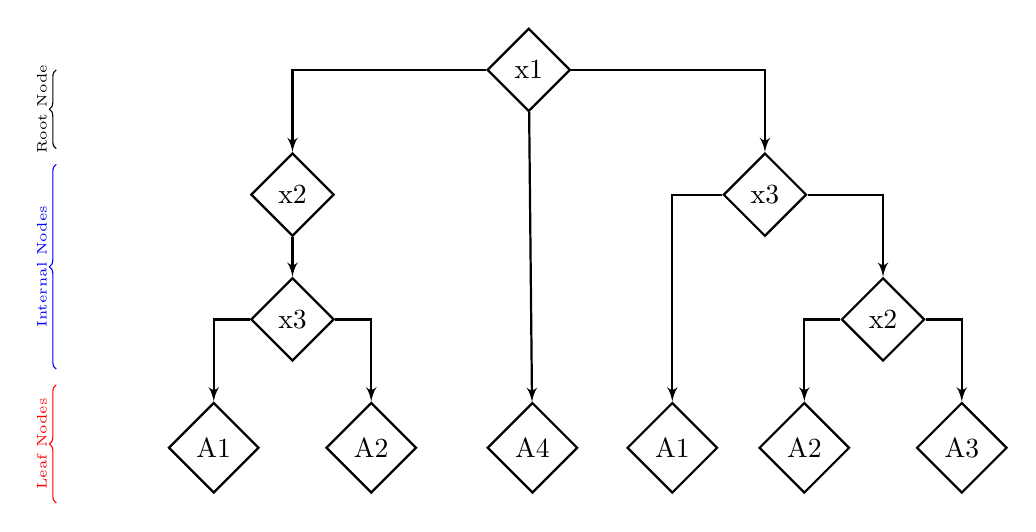
\begin{tikzpicture}[auto]
        \node [box]                                    (x3)      {x\ped{1}};
        \node [box, below=0.5cm of x3, xshift=-3cm]    (x1sx)    {x\ped{2}};
        \node [box, below=0.5cm of x3, xshift=3cm]     (x2dx)    {x\ped{3}};
        \node [box, below=0.5cm of x1sx]               (x2sx)    {x\ped{3}};
        \node [box, below=0.5cm of x2sx, xshift=1cm]   (A2sx)    {A\ped{2}};
        \node [box, below=0.5cm of x2sx, xshift=-1cm]  (A1sx)    {A\ped{1}};
        %\node [box, right=1cm of A2sx]                 (A3sx)    {A\ped{3}};
        %
        \node [box, below=0.5cm of x2dx, xshift=1.5cm]   (x1dx)    {x\ped{2}};
        \node [box, below=0.5cm of x1dx, xshift=-1cm]  (A2dx)    {A\ped{2}};
        \node [box, below=0.5cm of x1dx, xshift=1cm]   (A3dx)    {A\ped{3}};
        \node [box, left=0.5cm of A2dx]                (A1dx)    {A\ped{1}};
        \node [box, left=0.6cm of A1dx]                (A4dx)    {A\ped{4}};
        %
        \draw[decorate,decoration={brace},black] (-6,-1.0) -- node[above,rotate = 90, pos=.5]{\tiny Root Node}(-6,0);
        \draw[decorate,decoration={brace},red] (-6,-5.5) -- node[above,rotate = 90, pos=.5]{\tiny Leaf Nodes}(-6,-4);
        \draw[decorate,decoration={brace},blue] (-6,-3.8) -- node[above,rotate = 90, pos=.5]{\tiny Internal Nodes}(-6,-1.2);
        \path [line] (x3)   -|       (x2dx);
        \path [line] (x3)   -|       (x1sx);
        \path [line] (x3)   --       (A4dx);
        \path [line] (x2dx) -|       (x1dx);
        \path [line] (x2dx) -|       (A1dx);
        \path [line] (x1dx) -|       (A2dx);
        \path [line] (x1dx) -|       (A3dx);
        \path [line] (x1sx) --       (x2sx);
        %\path [line] (x1sx) -|       (A3sx);
        \path [line] (x2sx) -|       (A1sx);
        \path [line] (x2sx) -|       (A2sx);
    \end{tikzpicture}
    \caption{Decision Tree Diagram}
    \label{fig:diagram_decision_tree}
\end{figure}
\begin{figure}[h]
    \centering
    \includegraphics[width=8cm]{figure/Decision_Tree.png}
    \caption{Decision Tree Diagram}
    \label{fig:diagram_decision_tree}
\end{figure}

There are multiple measures that can be used in step 1 and step 2 for choosing an optimal attribute in the root node and determine the best partition. For example, the ID3 \cite{quinlan1986induction} and CART\cite{breiman1984classification}, both are classic Decision-Tree algorithms, using the Information gain and Gini impurity as the measure respectively. These two criteria come from the Entropy Theory\cite{pal1991entropy} and are used in evaluating the attributes' entropy. 

Here are their formulas, assumes that the dataset has $C$ classes and $p_i$ is the probability of randomly select a sample of class $i$:
\begin{align*}
    \text{Information entropy (E):} \ \  E &= -\sum_{i}^C p_i \times log (p_i) \\
    \text{Gini Impurity (G):} \ \  G &= \sum_{i=1}^C p_i \times (1 - p_i)
\end{align*}
\end{comment}

\par\noindent\textbf{Random-Forest} is a machine learning algorithm proposed by Leo Breiman\cite{breiman2001random} in 2001. Instead of using one decision tree which is nonunique and may exhibits high variance, random forest generates a number of individual decision trees operating as a committee. Bootstrapping technique is used to train the individual decision trees in parallel on different sub datasets and features with random sampling with replacement. The final decision of classification is aggregated by voting and averaging. With the wisdom of crowds, random forest can easily overcome overfitting problem and reduce model bias caused by data imbalance, and thus shows good generalization. 


\begin{comment}
Following the bootstrap method, it randomly selects $k$ independent and identically distributed training subsets. Correspondingly, the random forest is constructed to generate $k$ different decision trees for different subsets. For each decision tree, it only uses a limited number of the features. These well-trained base classifiers can be used in predicting labels of testing set, by using the voting or averaging.

Because of its randomness and it is a combination of multiple Decision-Trees, it can overcome the problem that Decision-Tree is easily over-fitting. What's more, it can also reduce model bias caused by data imbalance to some extent.
\end{comment}

 
\par\noindent\textbf{Logistic model} is a generalized linear model which is widely used in data mining. It assumes that the dependent variable $y$ follows a Bernoulli distribution and introduces non-linear factors through the Sigmoid function:
$$    y = \frac{1}{1 + e^{-z}},$$ where  $z = \beta_0 + \beta_1 x_1 + \dots + \beta_n x_n$  and $n$ is the number of features.
 

Assumes that $y$ represents a binary outcome $\{0, 1\}$, and $X$ is an array of their features and $\beta_i$ is the coefficient of feature $x_i$ \cite{peduzzi1996simulation}. The coefficient in logistic regression is called \textit{log odds} and used in logistic regression equation for the prediction of the dependent variable $y$ from the independent variable $X$, let $p = P(y=1)$:
\begin{comment}
\begin{align*}
    log\left(\frac{p(y = 1)}{1 - p(y = 1)}\right) &= \beta_0 + \beta_1 x_1 + \dots + \beta_n x_n \\
    \frac{p(y = 1)}{1 - p(y = 1)} &= exp(\beta_0 + \beta_1 x_1 + \dots + \beta_n x_n) \\
    \frac{1 - p(y = 1)}{p(y = 1)} &= \frac{1}{exp(\beta_0 + \beta_1 x_1 + \dots + \beta_n x_n)} \\
    \frac{1}{p(y = 1)} &= 1 + \frac{1}{exp(\beta_0 + \beta_1 x_1 + \dots + \beta_n x_n)} \\
    p(y=1) &= \frac{exp(\beta_0 + \beta_1 x_1 + \dots + \beta_n x_n)}{1 + exp(\beta_0 + \beta_1 x_1 + \dots + \beta_n x_n)} \\   
\end{align*}
\end{comment}
\begin{align*}
    log\left(\frac{p}{1 - p}\right) = \beta_0 + \beta_1 x_1 + \dots + \beta_n x_n \Rightarrow p = \frac{exp(\beta_0 + \beta_1 x_1 + \dots + \beta_n x_n)}{1 + exp(\beta_0 + \beta_1 x_1 + \dots + \beta_n x_n)} \\
\end{align*}
In practice, Logistics Regression can be used in multiple aspects, for instance, advertising, disease diagnosis as it can provide the possibility of a user buying a certain product and the possibility of a certain patient suffering from a certain disease. In our case, we want to use the ``8+2" risk factors and resident's lifestyle factors as input and give out the probability of stroke incidence, which can provide a forward-looking prediction.

\begin{comment}
\subsection{Classification Strategy}
In solving a multi-class classification problem, converting it into multi-binary classifications is an intuitive way to simplify the computation. Generally speaking, there are two strategies in do the converting \cite{rifkin2004defense}:
\begin{enumerate}
    \setlength{\itemsep}{0pt}
    \setlength{\parsep}{0pt}
    \setlength{\parskip}{0pt}
    \item One-vs.-Rest (or One-vs.-All, OvR)
    \item One-vs.One (or OvO)
\end{enumerate}

For the ``One-vs.-rest", categories would be one-hot encoded. Rather than just building one multi-class model, OvR needs $n$ classifiers for $n$ categories. For each data-points, it gets $n$ labels from those classifiers. Then we would use the label with the highest score as the predicted label for this sample. This method is commonly used in those machine learning models that can predict the score for the prediction such as Logistic Regression, Random Forest.

The aim of ``One-vs.-One" is to construct multiple binary classifiers between any two types of samples. If we have $n$ categories, the OvO needs $\frac{n(n-1)}{2}$ classifiers in total and for each classifier, we would have a predicted label based on the classifier. Based on those labels for a sample, we can use the hard-voting or soft-voting to distinguish which class the sample is in. This strategy is commonly used in linear models like Support Vector Machines(SVM) and Decision trees.
\end{comment}

\subsection{Model's Interpretation}\label{Model's Interpretation}

The model's interpretability and explanations are crucial for the medical data analysis: the medical diagnosis system must be transparent, understandable, and explainable. Therefore, the doctor and the patient can know how the model makes decisions, which features are important, and how the features affect the model's result \cite{ahmad2018interpretable, molnar2020interpretable}. In this section, we mainly introduce the feature importance, permutation importance and SHAP value which can help interpret the model.
\\
\par\noindent\textbf{Feature importance}, also called as Gini importance or Mean Decrease Impurity (MDI)\cite{breiman2001random,archer2008empirical, scikit-learn}, is the average of node impurity decrease of each variable and weighted by the probability of the sample reaching to that node. For Random-Forest model, assumes that the response is $Y$ and to calculate the average variable importance of feature $X_i$ with $N$ trees:

$$Imp(X_i) = \frac{1}{N} \sum_{T=1}^{N} \sum_{j\in T: v(s_j)=X_m} p(j) \Delta i(s_j, j)$$

Where $p(j) \Delta i(s_j, j)$ is the weighted impurity decreases for feature $X_i$ in all nodes $j$, $p(j)$ is the probability of the sample reading to node ($p(j) = \frac{N_j}{N} = \frac{\text{the amount of samples reaching the node $j$}}{\text{total amount of samples}}$) and $i(s_j, j)$ is the impurity measure at node $j$ with split $s_j$. $v(s_j)$ is the variable used in the split $s_j$(split $s_j$ means the split at node $j$. Hence, $v(s_j) = X_m$ means at node $j$, the splitting identifier is variable $X_m$).

For the Decision-Tree model, it only contains one tree, that is, $N = 1$, and its feature importance can be rewritten as:

$$Imp(X_i) = \sum_{v(s_j)=X_m} p(j) \Delta i(s_j, j)$$
\\
\par\noindent\textbf{Permutation Importance} \cite{breiman2001random,altmann2010permutation, fisher2019all,scikit-learn}, is used in answering how a certain feature influence the overall prediction, as it evaluates the changes of model prediction's accuracy by permuting the feature's values. If let $s$ represent the model accuracy with the full dataset $D$, then the permutation feature importance of $i^{th}$ feature  is:

$$Per_{Imp}(i) = s - \frac{1}{K} \sum_{j=1}^K s_{i, j}, $$
where $j$ represents the $j^{th}$ repetition in $K$ times shuffling for $i^{th}$ feature  , $s_{i, j}$ as the model accuracy in modified dataset $\hat{D}_{i, j}$ with $i^{th}$ feature  shuffled. With the average changed accuracy before and after shuffling can we evaluate the importance of $i^{th}$ feature.

% \begin{algorithm}[H]
% \caption{Permutation Importance}
% \begin{algorithmic}[1]
%     \SetAlgoLined
%     \State \textbf{INPUT}: trained model: $m$, dataset: $\mathcal{D}$\;
%     \State compute the accuracy of the model: $s$ (of the model $m$ on dataset $\mathcal{D}$)\;
%     \For{feature $i$ in $D$}{
%         \For{$j$ in $K$ ($K$ repetition)}{
%              Shuffle the column $i$ randomly and generate a new dataset $\hat{D}_{i, j}$\;
%              Compute the score $s_{i, j}$ \;
%         }
%      Compute the importance $I_j$ for feature $i$: $i_j = s - \frac{1}{K} \sum_{k=1}^K s_{i, j}$\;
%   }
% \end{algorithmic}
% \end{algorithm}



These two importance values can show which feature is more important, however, it is unavailable for us to know whether the feature has a positive or negative effect respect to the output.


\par\noindent\textbf{SHAP(Shapley Additive explanations)} can provide not only the importance of the features but also
show how much each feature contributes, either positively or negatively, to the target variable.
 It is a method to explain each individual prediction. This idea of SHAP value comes from the Shapley value in game theory. Shapley value tells how to fairly distribute the contributions among the features, which is the marginal contributions for each feature\cite{shap1953definition}. 
% The equation of Shapely value is shown below.
% \begin{equation}
%     g\left( z' \right)={{\phi }_{0}}+\sum\limits_{j=1}^{M}{{{\phi }_{j}}z_{j}^{'}} \\ 
% \end{equation}
% which $g$ is the explanation model,$z' \in \{0,1\}^{M}$ is the coalition feature vector, $M$ is the maximum coalition feature size and $\phi_j \in \mathbf{R}$ is the feature attribution for a feature j\cite{shap2017interpretation}.

The goal of SHAP is to explain the prediction of an instance ${x}^{i}$ by computing the contribution of each feature to the prediction model. The formula of SHAP is an addictive feature attribution linear model, and it is shown below:
\begin{equation}
    {{\phi }_{i}}=\sum\limits_{S\subseteq F\backslash{\{{x}^{i}\}}}{\frac{|S|!(n-|S|-1)!}{n!}}\left[v(S\cup \{{x}^{i}\})-v(S)\right] 
\nonumber\end{equation}
 with  $ S\subseteq \{{{x}^{1}},{{x}^{2}},\cdots ,{{x}^{n}}\}\backslash {{x}^{i}},F = \{{{x}^{1}},{{x}^{2}},\cdots ,{{x}^{n}}\}.$
 
 With this method, we calculate how the feature contributes to each coalition of each decision tree model and sum them up to get the total contribution of the whole prediction model. In this equation, $F\backslash{\{{x}^{i}\}}$ represents all the possible subsets without feature ${x}^{i}$, $S$ represents the sub-feature set that did not contain the result, $v(S\bigcup \{{x}^{i}\})$ represents the model output (precision, recall or accuracy, etc.) after feature ${x}^{i}$ is added to subset $S$, $v(S)$ represents the model output using subset $S$. With the multiplication for the occurrence probability for each subsets without that feature and the output different with and without that feature, the marginal contribution of each feature ${x}^{i}$ is calculated.
 
 SHAP has three properties: local accuracy, missingness, and consistency \cite{shap2017interpretation}. Local accuracy means that when approximating the original model for a specific input $x$, local accuracy requires the explanation model to at least match the output of the model for the simplified input $x'$. Missingness means that if there is a feature missing in the sample, it does not affect the output of the model. Consistency means that when the model changes and the marginal contribution of a feature increases, the corresponding Shapley value will also increase. Therefore, it is more accurate and scientific in interpreting machine learning models due to those three characteristics.

\section{Result}\label{section:results}
\subsection{Main Risk Factors Ranking}
 Due to geographic and cultural differences, the same disease may have different manifestations in different region. We hope to find the topmost influential factors in Shanxi Province. Table \ref{table:Risk-factor-exposure} shows the proportion of each risk factor's Exposure rate and the Risk attribution (RA) based on our data:
 \footnote{
\begin{align*}
    \text{Exposure rate} &= \frac{\text{Number of patients for specific disease}}{\text{Total number in dataset}} \\ 
    \text{Risk attribution} &= \frac{\text{Incidence of a specific disease in patients has history of stroke}}{\text{Incidence of a specific disease in has no history of stroke}}
\end{align*}}
\begin{table}[H]
\small
\centering
\begin{tabular}{ccc}
\hline
\multicolumn{1}{c}{\textbf{Feature}}&\multicolumn{1}{c}{\textbf{Exposure rate}} & \multicolumn{1}{c}{\textbf{Risk attribution}}\\ \hline
Hypertension                & 0.5158  & 1.187  \\
Hyperlipidemia              & 0.3765  & 0.5846 \\
Physical Inactivity         & 0.3892  & 1.721  \\
Overweight                  & 0.3373  & 0.6844 \\
Smoking                     & 0.2058  & 1.539  \\
Family history of stroke    & 0.0999  & 1.590 \\
Diabetes Mellitus           & 0.0709  & 2.613 \\
History of stroke           & 0.0483  & NA \\
Heart Disease               & 0.0052  & 11.84 \\
History of TIA              & 0.0023  & NA  \\ \hline
\end{tabular}
\caption{Main Risk Factor Exposure rate and Risk attribution} \label{table:Risk-factor-exposure}
\end{table}

To assess the ranking of main risk factors, in the first experiment, we used the dataset 2 with the ``8+2'' factors as feature and implemented the Decision-Tree model.  Table \ref{table:DT-main-factor} shows the classification result:
\begin{table}[H]
\small
\centering
\begin{tabular}{ccccc}
\hline
\textbf{}    & \textbf{precision} & \textbf{recall} & \textbf{f1-score} & \textbf{support} \\ \hline
Low risk     & 0.9707             & 0.9950             & 0.9827            & 1999           \\
Mid risk     & 0.9711             & 0.9411          & 0.9599            & 1313           \\
High risk    & 0.9751                & 0.9650          & 0.9678            & 1345           \\
accuracy     &                    &                 & 0.9721            &                  \\
macro avg    & 0.9794             & 0.9787          & 0.9789            & 4657           \\
weighted avg & 0.9799             & 0.9796          & 0.9795            & 4657           \\ \hline
\end{tabular}
\caption{Result of Decision Tree model} \label{table:DT-main-factor}
\end{table}

Figure \ref{fig:feature_permutation_10_factor} shows the feature importance and permutation importance based on the Decision Tree model, which \textcolor{violet}{shows the ranking of these main risk factors: both evaluation methods confirm that hypertension, physical inactivity, and hyperlipidemia are estimated as the top three informative features in the Decision-Tree model.} 

\begin{figure}[H]
\centering
\begin{minipage}[t]{0.48\textwidth}
\centering
\includegraphics[width=8cm]{figure/feature_importance_eight_two.png}
%\caption{Feature Importance}
\end{minipage}
\begin{minipage}[t]{0.48\textwidth}
\centering
\includegraphics[width=8cm]{figure/permutation_importance_eight_two.png}
%\caption{Permutation Importance}
\end{minipage}
\caption{Feature and Permutation Importance of ``8+2" Risk factor}\label{fig:feature_permutation_10_factor}
\end{figure}


\subsection{Lifestyle and Medical Measurement Ranking}
For the second experiment, we would like to identify  
more risk factors for Shanxi Province besides the "8+2" risk factors by using the dataset 2 with features such as lifestyle habits and medical measurement.
Table \ref{table:RF-lf-mm-factors} shows the classification result and Figure \ref{fig:feature_permutation_10_factor_life_med} shows the feature and permutation importance:
\begin{table}[H]
\small
\centering
\begin{tabular}{ccccc}
\hline
\textbf{}    & \textbf{precision} & \textbf{recall} & \textbf{f1-score} & \textbf{support} \\ \hline
Low risk     & $0.8007(\pm 0.007)$             & $0.9531(\pm 0.004)$          & $0.8703(\pm 0.0041)$            & $1962$           \\
Mid risk     & $0.8213(\pm 0.008)$             & $0.7850(\pm 0.011)$          & $0.7901(\pm 0.0064)$               & $1367$           \\
High risk    & $0.9124(\pm 0.013)$             & $0.7182(\pm 0.010)$          & $0.8026(\pm 0.0076)$         & $1426$           \\
accuracy     &                    &                 & $0.84 (\pm 0.01)$            &                  \\
macro avg    & $0.8421(\pm 0.0081)$             & $0.8179(\pm 0.011)$          & $0.8271(\pm 0.0034)$            & $4755$           \\
weighted avg & $0.8311(\pm 0.0095)$             & $0.8400(\pm 0.010)$          & $0.8344(\pm 0.0062)$            & $4755$           \\ \hline
\end{tabular}
\caption{Result of Decision Tree model} \label{table:RF-lf-mm-factors}
\end{table}

 The results shown in Figure \ref{fig:feature_permutation_10_factor_life_med} confirm  that systolic blood pressure, diastolic blood pressure, physical inactivity, BMI, smoking, FBG, TG, HDL, family history of Stroke and weight are the top ten factors when we only consider the lifestyle habits, demographic information, and medical measurement. These factors are, medically, highly corresponding to the Chronic diseases \cite{levy2009genome, decode2001glucose, wu2007cut}.  
\begin{figure}[H]
\centering
\begin{minipage}[t]{0.48\textwidth}
\centering
\includegraphics[width=8cm]{figure/feature_importance_others.png}
\caption{Feature Importance}
\end{minipage}
\begin{minipage}[t]{0.48\textwidth}
\centering
\includegraphics[width=8cm]{figure/permutation_importance_others.png}
\caption{Permutation Importance}
\end{minipage}
\caption{Feature and Permutation Importance of lifestyle and medical measurement factors factor}
\label{fig:feature_permutation_10_factor_life_med}
\end{figure}

To give out the specific details on how each feature contributes to each individual, we calculate the SHAP value in the Random Forest model and use the summary-plot to show their importance. The figure of ordered mean sample SHAP value for each feature is shown in Figure \ref{fig:shap_value}. It shows the distribution of the contributions each factor has on the cause of stroke. The color represents the feature value (red  represents  high, blue  represents  low). The more difference for the distribution between high feature value and low feature value, the better it would be in separating patients with different risk levels.  Figure \ref{fig:shap_value} shows that Diastolic Blood Pressure, Physical inactivity, Systolic Blood Pressure, BMI, Smoking, FBG, and TG are positively correlated to the risk of stroke, and HDL are negatively correlated to the risk. 
\begin{figure}[H]
    \centering
    \includegraphics[width=10cm]{figure/shapley_value.png}
    \caption{TreeSHAP value of top lifestyle and medical measurement factors factors}
    \label{fig:shap_value}
\end{figure}

\subsection{Quantitative Prediction of Stroke's Incidence}
For the third experiment, 
a logistic model is 
 establish to  quantify the probability of stroke incidence.  To achieve this goal, we combine the dataset 1 and 2,  relabel the data: the original low-risk and medium-risk are now class 0, the high-risk and stroke are class 1. The features contains lifestyle information, demographic information, and the ``8+2" factors.
% , as they are easily accessible and residents are able to use this model as a preliminary check by themselves.

 Logistic regression is feature-sensitive.  Feature selection is done before modeling. To solve the multicollinearity problem \cite{alin2010multicollinearity},   the highly relevant features are removed first. For example, we keep BMI and remove height and weight. What's more,   Variance Threshold \cite{guyon2003introduction} is used to remove low variance features. It is a simple method of feature selection, where deletes all the features whose variance does not meet a certain threshold. For example, most of the respondent in our survey are Han Chinese, therefore, we remove ethnicity.
 
 The logistic model results are shown in Table \ref{table:logistic-factor}   including the features' coefficient, standard error, and the confidence interval. 
 %Figure \ref{fig:feature-effect-logit}
 According to the coefficients, it yields that History of stroke, Physical inactivity,  Hypertension, Hyperlipidemia, Smoke, Diabetes Mellitus, BMI, Family history of stroke and Heart disease are positive correlated to stroke incidence; Education level, Frequency of vegetables, and Occupation are negative correlated to stroke incidence.  
\begin{table}[H]
\small
\centering
\begin{tabular}{ccccccc}
\hline
\textbf{y=1}             & \textbf{coef} & \textbf{std err} & \textbf{z} & \textbf{$P >|z|$} & \multicolumn{2}{c}{\textbf{95\% CI {[}0.025, 0.975{]}}} \\ \hline
History of Stroke        & 2.6779  & 0.247 & 10.853  & 0.000 & 2.194  & 3.162  \\
Physical Inactivity      & 1.3948  & 0.027 & 50.815  & 0.000 & 1.341  & 1.449  \\
Hypertension             & 1.1489  & 0.027 & 41.970  & 0.000 & 1.095  & 1.203  \\
Hyperlipidemia           & 1.0875  & 0.025 & 43.210  & 0.000 & 1.038  & 1.137  \\
Smoke                    & 1.0455  & 0.031 & 33.892  & 0.000 & 0.985  & 1.106  \\
Diabetes Mellitus        & 0.8043  & 0.025 & 32.525  & 0.000 & 0.756  & 0.853  \\
BMI                      & 0.7897  & 0.026 & 30.635  & 0.000 & 0.739  & 0.840  \\
Family history of stroke & 0.7447  & 0.024 & 30.522  & 0.000 & 0.697  & 0.793  \\
Heart Disease            & 0.4257  & 0.029 & 14.630  & 0.000 & 0.369  & 0.483  \\
Frequency of Fruit       & 0.1507  & 0.026 & 5.817   & 0.000 & 0.100  & 0.202  \\
Alcohol                  & 0.1325  & 0.025 & 5.198   & 0.000 & 0.083  & 0.182  \\
Pulse                    & 0.1279  & 0.023 & 5.606   & 0.000 & 0.083  & 0.173  \\
Sex                      & 0.0863  & 0.029 & 2.945   & 0.003 & 0.029  & 0.144  \\
Retire                   & 0.0754  & 0.025 & 3.015   & 0.003 & 0.026  & 0.125  \\
Age                      & 0.0548  & 0.026 & 2.084   & 0.037 & 0.003  & 0.106  \\
Frequency of Vegetables  & -0.2262 & 0.025 & -9.118  & 0.000 & -0.275 & -0.178 \\
Occupation               & -0.2166 & 0.026 & -8.308  & 0.000 & -0.268 & -0.165 \\
Education Level          & -0.3640 & 0.027 & -13.604 & 0.000 & -0.416 & -0.312 \\
constant                 & -0.7868 & 0.068 & -11.545 & 0.000 & -0.920 & -0.653 \\ \hline
\end{tabular}
\caption{Features' Coefficient and Confidence Interval}
\label{table:logistic-factor}
\end{table}

% \begin{figure}[H]
%     \centering
%     \includegraphics[width=15cm]{figure/logit_feature_importance.png}
%     \caption{Logistic Model's Feature Importance}
%     \label{fig:feature-effect-logit}
% \end{figure}

 The trained model is implemented on the testing set  to estimate the probability of stroke incidence for each category. The results are in Table \ref{table:average_stroke_probability}:

\begin{table}[H]
\small
\centering
\begin{tabular}{cc}
\hline
\textbf{Risk   Level} & \textbf{Average Probability of Stroke} \\ \hline
Low                   & $0.0720 \ (95\% CI: (0.0665, 0.0774))$                                \\ 
Medium                & $0.1902 \ (95\% CI: (0.1808, 0.1996))$                                \\ 
High                  & $0.8389 \ (95\% CI: (0.8293, 0.8486))$                                \\ \hline
\end{tabular}
\caption{The average stroke probability for each risk level based on Logistic Model}
\label{table:average_stroke_probability}
\end{table}

Comparing with the  qualitative  ranking method, we quantify the risk factors of stroke, and convert the scoring grades into probabilities, making the prediction of stroke risk more intuitive. What's more,  our logistic model is based on the current actual circumstance to predict the incidence promptly, which is more time-sensitive. 


\section{Discussion}\label{section:dicuss}
\subsection{The Risk Factors in Shanxi Province}
Based on the treeSHAP value, feature and permutation importance of lifestyle and medical measurement, we have found the most important factors of causing   stroke: 
\begin{enumerate}
    \setlength{\itemsep}{0pt}
    \setlength{\parsep}{0pt}
    \setlength{\parskip}{0pt}
    \item Hypertension(Diastolic Blood pressure and Systolic Blood Pressure)
    \item Physical Inactivity
    \item Overweight (BMI)
    \item Hyperlipidemia (mostly according to the HDL and TC)
    \item Diabetes Mellitus (according to the FBG)
\end{enumerate}


% to Systolic Blood Pressure, Diastolic Blood Pressure might be better in diagnosing the risk of patients getting a stroke. Based on the dependence plot in Figure \ref{fig:diastolic_shap}, we can see that diastolic blood pressure
 The treeSHAP dependence plot is applied to compare the contribution between two features. 
 %It is a scatter plot showing the effect of a specific feature has on the predictions made by the model. 
 Figure \ref{fig:diastolic_shap} shows that Diastolic Blood Pressure ($>$ 140 mmHg) is more suitable in diagnosing the risk of patients getting a stroke than the Systolic Blood Pressure ($>$ 90 mmHg). 
 %Diastolic Blood pressure  contributes more a lot to diagnosing patients with high diastolic blood pressure($>$ 140 mmHg) comparing to patients with high systolic blood pressure($>$ 90 mmHg).
 Similarly, based on the comparison between HDL and LDL (see Figure \ref{fig:HDL_shap}), we can find that high-density lipoprotein are better in diagnosing those non-stroke patients in low high-density lipoprotein.
\begin{comment}
Comparing to Systolic Blood Pressure, Diastolic Blood Pressure might be better in diagnosing the risk of patients getting a stroke. Based on the dependence plot in Figure \ref{fig:diastolic_shap}, we can see that diastolic blood pressure contributes more a lot to diagnosing patients with high diastolic blood pressure($>$ 140 mmHg) comparing to patients with high systolic blood pressure($>$ 90 mmHg). Similarly, based on the comparison between HDL and LDL (see Figure \ref{fig:HDL_shap}), we can find that high-density lipoprotein are better in diagnosing those non-stroke patients in low high-density lipoprotein.
\end{comment}
\begin{figure}[H]
\centering
\begin{minipage}[t]{0.48\textwidth}
\centering
\includegraphics[width=8cm]{figure/diastolic_shapley_value.png}
\caption{Dependence Plot for Systolic Blood Pressure and Diastolic Blood Pressure}
\label{fig:diastolic_shap}
\end{minipage}
\begin{minipage}[t]{0.48\textwidth}
\centering
\includegraphics[width=8cm]{figure/HDL_shapley_value.png}
\caption{Dependence Plot for HDL and LDL}
\label{fig:HDL_shap}
\end{minipage}
\end{figure}

%\subsection{Comparison between 2016 data and 2017-2020 data} \label{comparison:2016-others}
%\textcolor{violet}{In section \ref{section:results}, we use dataset 1 and dataset 2 in modelling and ranking. In this section, we compare the dataset 2 with an additional dataset: 2016 census data. We call it dataset 3.} This dataset has these three problems:
%\begin{itemize}[leftmargin=10pt]
%     \setlength{\itemsep}{0pt}
%     \setlength{\parsep}{0pt}
%     \setlength{\parskip}{0pt}
%     \item[1.] Data sources are very limited, and the surveyed communities are mainly concentrated in Taiyuan City
%     \item[2.] Data is imbalanced (Low-risk: Medium-risk: High-Risk = 1515: 429: 321)
%     \item[3.] \textcolor{violet}{The size of data set 3 is smaller than dataset 2}
% \end{itemize}

% By visualizing the geographic distribution of the respondents \footnote{by using a Open Source GIS software: \href{https://qgis.org/en/site/}{QGIS} with \href{https://www.openstreetmap.org}{Open Street Map} and \href{http://datav.aliyun.com/tools/atlas/}{DATAV.GeoAtlas} provides the GeoJson of Shanxi Province} (shown in Figure \ref{fig:map}), we can see that the residential area in dataset 3 is relatively narrow and the number of people covered is smaller than the dataset 2 (the green circle represents the 2016 data's location and the red triangle represents the 2017-2020 data's) which may lead an issue of lacking feature diversity. 

% \begin{figure}[H]
%     \centering
%     \includegraphics[width=5cm]{figure/map.png}
%     \caption{Geographical Visualization}
%     \label{fig:map}
% \end{figure}

% \textcolor{violet}{We implement the One-factor ANOVA\cite{mendenhall2012introduction} on both dataset 3 and dataset 2. by comparing the means of two groups (medium-risk and high-risk) and identify whether they are statistical significant.} Table \ref{table:one-factor-anova} shows that over $70\%$ features in dataset 3 have no significant difference between the medium level and high level when considering the linear relationship. (with probability level 0.05). 
% \begin{enumerate}
%     \setlength{\itemsep}{0pt}
%     \setlength{\parsep}{0pt}
%     \setlength{\parskip}{0pt}
%     \item Null Hypothesis: the feature has no significant difference in mid-risk and high-risk ($\mu_{\text{mid}}= \mu_{\text{high}}$)
%     \item Alternative Hypothesis: the feature has significant difference in mid-risk and high-risk ($\mu_{\text{mid}} \neq \mu_{\text{high}}$)
% \end{enumerate}

% \begin{table}[H]
% \centering
% \scalebox{0.7}{\begin{tabular}{lll}
% \\ \hline
% \textbf{Feature name}                                & \textbf{p-value in 2016 data}          & \textbf{p-value in 2017-2020 data}    \\ \hline
% first Systolic Blood Pressure                        & 0.953135801                            & 5.98E-18                              \\
% LDL                                                  & 0.949184631                            & 1.07E-07                              \\
% second Systolic Blood Pressure                       & 0.897969538                            & 1.14E-12                              \\
% Frequency of Eating Fruit                            & 0.870816774                            & 0.020469893                           \\
% First Pulse Rate                                     & 0.868571233                            & 0.804459134                           \\
% TC                                                   & 0.792057452                            & 0.386549146                           \\
% Second Pulse Rate                                    & 0.774606567                            & 0.159667209                           \\
% CAS                                                  & 0.770795895                            & 7.76E-22                              \\
% Meat and Vegetable                                   & 0.730663135                            & 0.000101384                           \\
% Second Diastolic Blood Pressure                      & 0.693464907                            & 0.185422092                           \\
% Education Level                                      & 0.693318513                            & 0.403905044                           \\
% FBG                                                  & 0.68401876                             & 7.59E-26                              \\
% First Diastolic Blood pressure                       & 0.594867705                            & 0.415466006                           \\
% Income                                               & 0.5254845                              & 0.318749163                           \\
% PCI                                                  & 0.38738746                             & 7.88E-20                              \\
% CABG                                                 & 0.38738746                             & 3.35E-20                              \\
% Frequency of Eating Vegetable                        & 0.333279583                            & 0.050297245                           \\
% Living Condition                                     & 0.296975766                            & 1.10E-06                              \\
% Ethnicity                                            & 0.291471954                            & 0.477784183                           \\
% Marital Status                                       & 0.227514649                            & 0.001039285                           \\
% GHb                                                  & 0.169449648                            & 1.55E-32                              \\
% HCY                                                  & 0.091474934                            & 2.84E-09                              \\
% Occupation                                           & 0.067473416                            & 0.000272427                           \\
% Sex                                                  & 7.34E-05                               & 2.82E-87                              \\
% Alcohol                                              & 6.13E-05                               & 0.0*                                  \\
% Retire                                               & 2.95E-05                               & 0.23891555                            \\
% Age                                                  & 8.43E-06                               & 3.37E-12                              \\
% Waistline                                            & 1.41E-06                               & 1.67E-197                             \\
% TG                                                   & 1.42E-07                               & 9.08E-202                             \\
% HDL                                                  & 3.31E-09                               & 7.47E-106                             \\
% BMI                                                  & 1.01E-12                               & 2.76E-227                             \\ \hline
% \end{tabular}}
% \caption{One-Factor ANOVA}
% \label{table:one-factor-anova}
% \end{table}

% We also use a random-forest model to check whether the features is dataset 3 have some non-linear relationship. Table \ref{table:comparison} shows the result. By comparing with the dataset 2's random-forest result, the random-forest model does not perform well in dataset 3.
% \begin{table}[H]
% \centering
% \begin{tabular}{|l|l|l|l|l|l|l|}
% \hline
% & \multicolumn{2}{l|}{{Low}} & \multicolumn{2}{l|}{{Mid}} & \multicolumn{2}{l|}{{High}} \\ \hline
% & Precision         & Recall      & Precision           & Recall        & Precision    & Recall        \\ \hline
% 2016 data & 0.80    & 0.99        & 0.78                &0.48           & 0.72         &0.29        \\ \hline
% dataset 2 & 0.80    & 0.95        & 0.82                & 0.79          & 0.91         & 0.72           \\ \hline
% \end{tabular}
% \caption{Comparison between 2016 and 2017-2020's result}
% \label{table:comparison}
% \end{table}

% This result may caused by the data imbalance problem. Therefore, we propose a new model with two commonly used classification strategies\cite{rifkin2004defense}: 

% \begin{enumerate}
%     \setlength{\itemsep}{0pt}
%     \setlength{\parsep}{0pt}
%     \setlength{\parskip}{0pt}
%     \item One-vs.-Rest (or One-vs.-All, OvR)
%     \item One-vs.One (or OvO)
% \end{enumerate}

% The idea is to divide this multi-class classification into two binary classifications and these two classifiers are serial. Instead of using only OvR or OvO, we use both of these strategies and converting the problem into step-by-step binary classification problem. We call this strategy \textit{pipeline strategy} and its flow chart is shown in Figure \ref{fig:pipeline-model}:
% \begin{figure}[H]
%     \centering
%     \includegraphics[width=8cm]{figure/Pipeline_Model.PNG}
%     \caption{Multi-class classification with pipeline strategy}
%     \label{fig:pipeline-model}
% \end{figure}

% In general, this strategy separates the multi-class classification into two steps:
% \begin{itemize}
%     \setlength{\itemsep}{0pt}
%     \setlength{\parsep}{0pt}
%     \setlength{\parskip}{0pt}
%     \item[1.]  Using Classifier 1 to classify the low-risk and the others(medium-risk and high-risk).
%     \item[2.]  Using Classifier 2 to classify the medium-risk and high-risk. 
% \end{itemize}
% For the classifier 1, as it combines the medium-risk and high-risk group, the imbalanced ratio can be decreased, which can help solving the model bias problem. Table \ref{table:pipline_result} shows the  comparison between normal random-forest and random-forest with pipeline strategy. With the pipeline strategy, the classification result has a great improvement.

% \begin{table}[H]
% \centering
% \begin{tabular}{|l|l|l|l|l|l|l|}
% \hline
%  2016 data         & \multicolumn{2}{l|}{{Low}} & \multicolumn{2}{l|}{{ Mid}} & \multicolumn{2}{l|}{{High}} \\ \hline
%           & Precision                & Recall               & Precision                & Recall               & Precision                & Recall                \\ \hline
% One-vs.Rest & 0.80                      & 0.99                 & 0.78                     & {0.48}                 & 0.72                     & {0.29}                  \\ \hline
% Pipeline Strategy &0.86                     & 0.86                 & 0.64                     & 0.58                & 0.65                     & 0.70               \\ \hline
% \end{tabular}
% \caption{Comparison of One-vs.Rest and Pipeline Strategy}
% \label{table:pipline_result}
% \end{table}


\subsection{Feature Validity}
Missing data due to the technique errors (like typos and facilities errors) is a common problem during  the census analysis. To find out how might those error data in the datasets might influence, we have conducted an experiment to find out missing data in features and its influence on the final results.  The Random Forest Classifier is adopted to predict the stroke risk  with different proportions of a single missing feature and looped for 100 times
at random locations.  What's more, to prevent the precision score didn't change due to the strong-correlation of features, some specific feature pairs are cleaned up. The result is shown in Figure \ref{fig:feature_valid} :

\begin{figure}[H]
    \centering
    \includegraphics[width=8cm]{figure/Feature_Validity.png}
    \caption{The relationship between the proportion of missing data in feature and the weighted precision score}
    \label{fig:feature_valid}
\end{figure}

In Figure \ref{fig:feature_valid}, the curve for each feature represents how the average weight precision score of the feature has changed with the increasing proportion of the feature missing and the shadows are the 95\% confidence area 100 times for each feature. Based on the result, we can see that diastolic blood pressure, physical inactivity, BMI, smoking, alcohol, HDL, and FBG are in order important factors when identifying the cause of stroke, while the other factors are not influencing the whole models. An interesting fact we have seen is that HDL seems to be a great influential factor when the proportion of HDL is small compared to most of the influenced factors.

What's more, a Recursive Feature Elimination (RFE) process is also done to evaluate the specific amount of factors for analyzing the risk level of patients getting a stroke. The procedure of the RFE is as follows. First, the estimator is trained on the initial feature set and the importance of each feature is obtained from any specific or callable attribute. Then, the least important features are removed from the current feature set. This process is repeated recursively over the pruning set until the number of features to be selected is finally reached. Based on the Figure \ref{fig:feature_valid_precision}, we have found that approximate 7 features can help the Random Forest model to get a stable precision for different levels of risk. Therefore, the validity of those features is proved.
\begin{figure}[H]
    \centering
    \includegraphics[width=10cm]{figure/precision_feature_valid.png}
    \caption{The relationship between the amount of features and the precision changed}
    \label{fig:feature_valid_precision}
\end{figure}

\bibliographystyle{unsrt}
\bibliography{reference}
\end{document}
